
 
\section{Experiments}

In this section, we demonstrate the performance of DenseBox on MALF(Multi-Attribute Labelled Faces) dataset\cite{faceevaluation15}  and KITTI\cite{Geiger2012CVPR} car detection task. We also evaluate our method on those tasks with or without the help of landmark annotation, showing that multi-task learning with landmark localization can significantly boost the performance. We compare our results with current the state-of-the-art systems, which shows that our method achieves competitive results on object detection tasks.  Nothe that we do not compare the performances of our DenseBox with original R-CNN directly on those task, but we highlight the performances of other methods which claim to use R-CNN or those methods have alrealy compared themselves to R-CNN. 

\subsection{ MALF  Detection Task}
The MALF detection test dataset contains 5,000 images in collected from the Internet. Unlike the widely used FDDB\cite{jain2010fddb} face detection benchmark, which is collected from news photos and the pose tends to be frontal, the face images in MALF have much larger diversity, making it closer to real world application than FDDB. 

\textbf{Training and Testing.} We train two models described in section \ref{sec:model} on 31,337 Internet-collected  images with  81,024 faces annotated with 72 landmarks illustrated in Fig \ref{fig:fig_landmark}. One model only use bounding box information, while the other model utilize both bounding box and landmark information for comparison. They are both initialized with ImageNet pre-trained VGG19 model.  The faces in training are roughly scaled to 50 pixels in height, and the scale jitter range is $[0.8,1.25]$ , the same as described in section \ref{sec:training}.  On testing, we first selectively down sample images so that for each image the longest image side does not exceed 800 pixels.  Then we test our model on each image at several scales.  The test scale starts from $2^{-3}$ to $2^{1.2}$ with the step of $2^{0.3}$. This setting enable our models to detect faces from 20 pixels to 400 pixels in height. The non-maximum suppression IOU threshold in face detection is set to $0.5$.  Under this configuration, it taks several seconds to process one image in MALF dataset on an Nvidia K40 GPU. 
	\begin{figure} 
	\centering
	 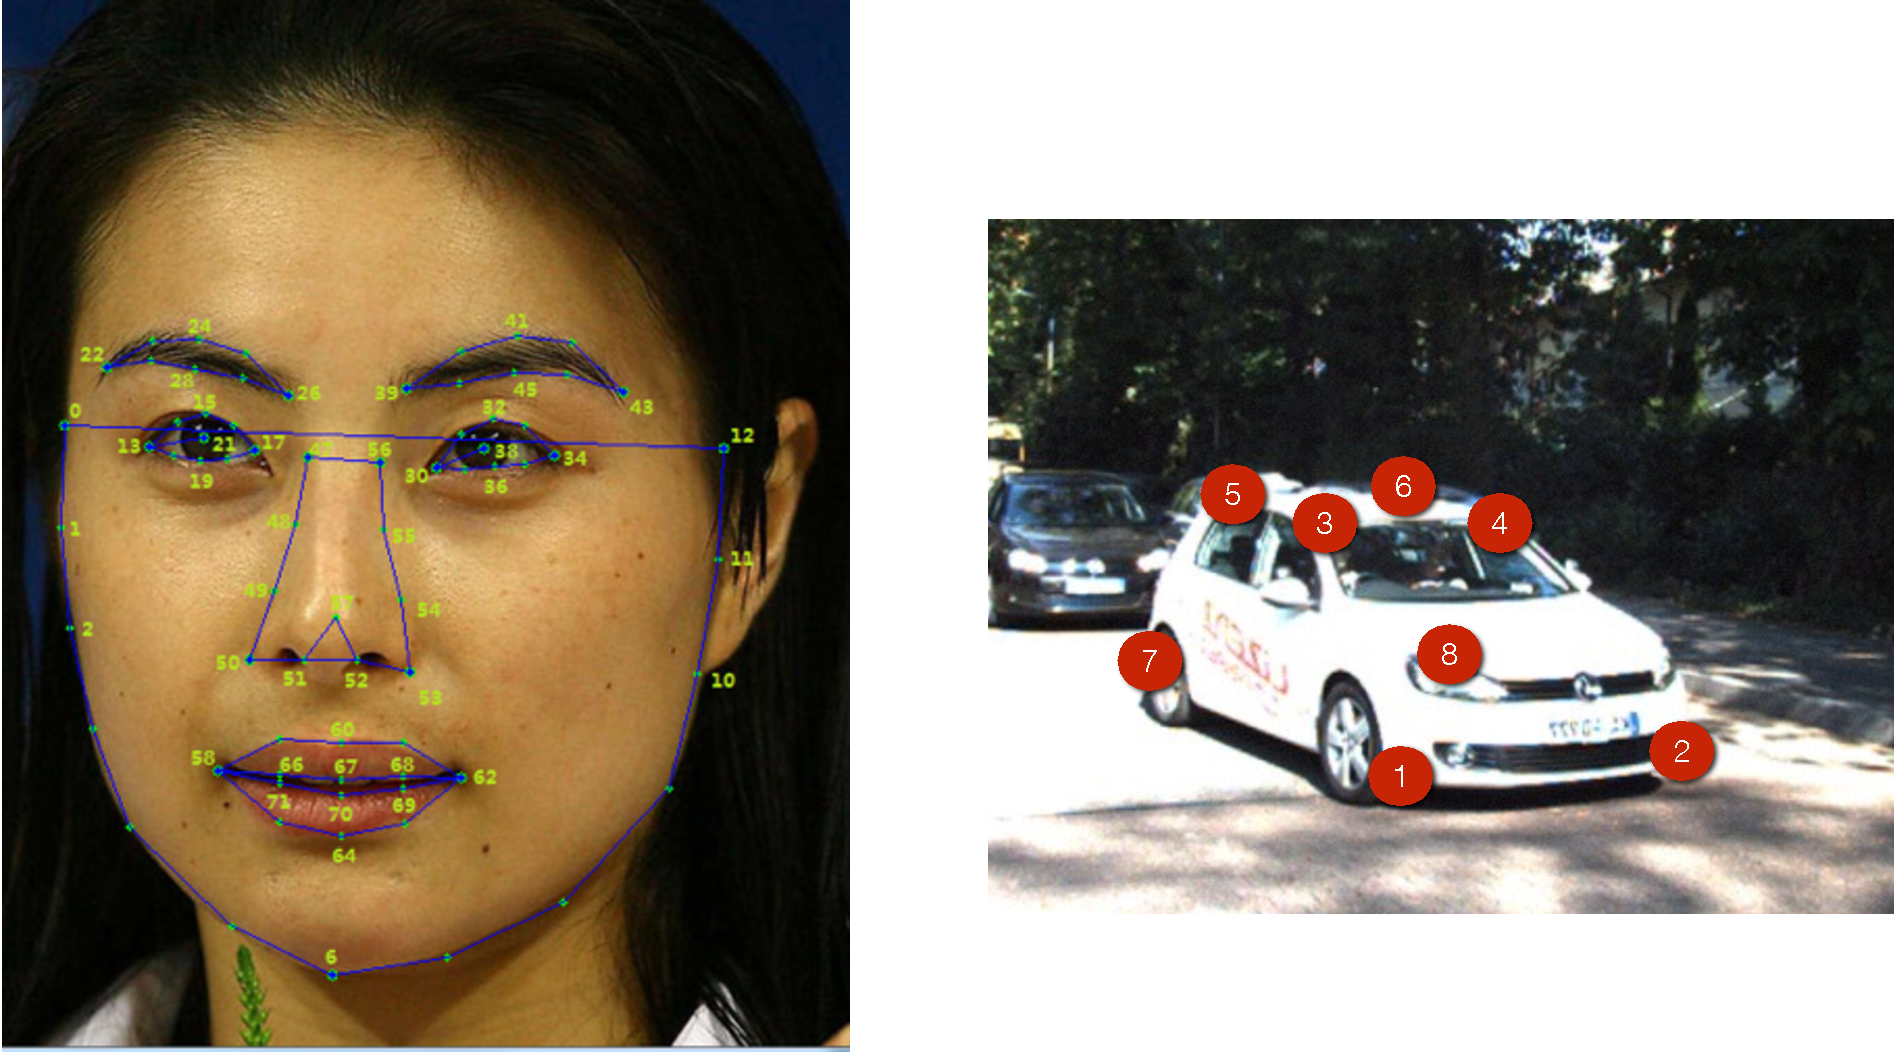
\includegraphics[scale=0.45]{figures/figure_landmark-crop.pdf}
	\caption{\textbf{Left: } 72 landmarks for face. \textbf{Right: } 8 landmarks for car. }
	\label{fig:fig_landmark}
	\end{figure}
\textbf{Results.} 
We illustrate the results of three versions of DenseBox on MALF dataset. The ``DenseBoxNoLandmark’’ denotes DenseBox without landmark in training. ``DenseBoxLandmark’’ is the model incorporating landmark localization, and ``DenseBoxEnsemble’’ is the result of ensembling 10 DenseBox with landmarks from different batch iterations. As shown in Fig \ref{fig:fig_malf}, landmark localization gives a significant performance boost on face detection.  We also notice that the models trained with different batch iterations still have high diversity since another significant boost has been seen by model ensemble. Then we compare our best model with other state-of-the-art methods on MALF. Surprisingly, our model achieves the best performance, with mean recall rate of $87.26\%$, almost outperform DDFD by $10\%$, which claims to have better performance than R-CNN on face detection task. 
 
 
\begin{figure} 
  \begin{minipage}[t]{0.5\linewidth} % 如果一行放2个图,用0.5,如果3个图,用0.33
    \centering 
    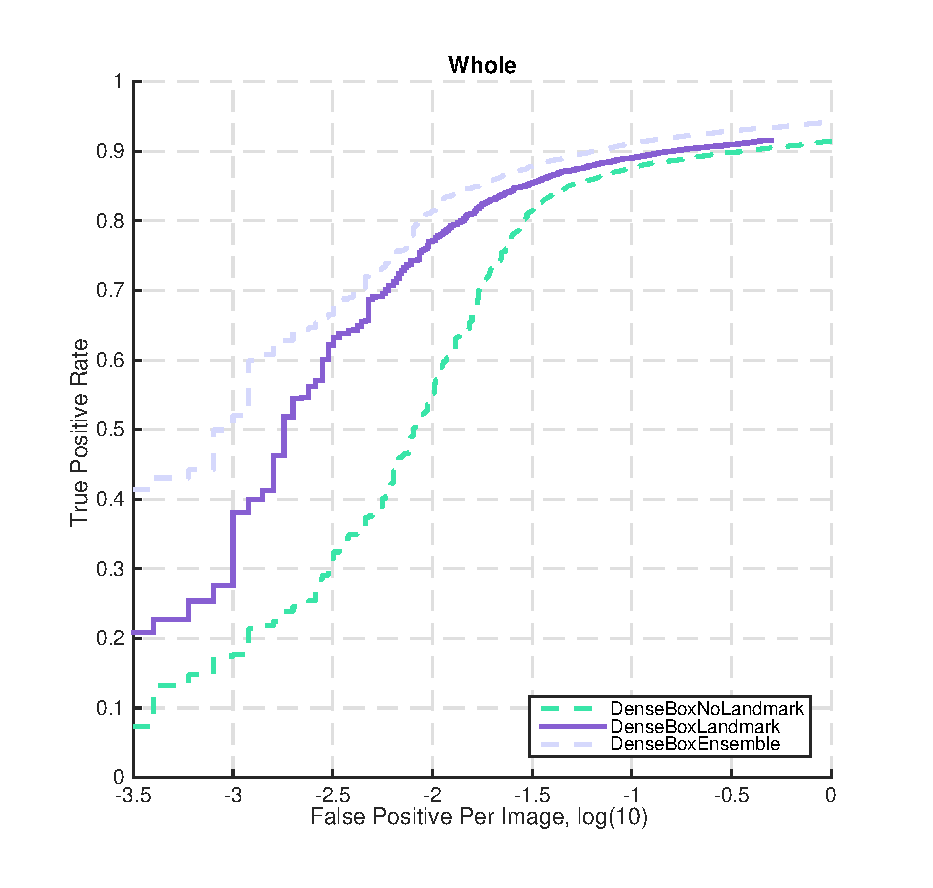
\includegraphics[scale = 0.5]{figures/MALF_1.eps}  (a)
  \end{minipage}% 
  \begin{minipage}[t]{0.5\linewidth} 
    \centering 
    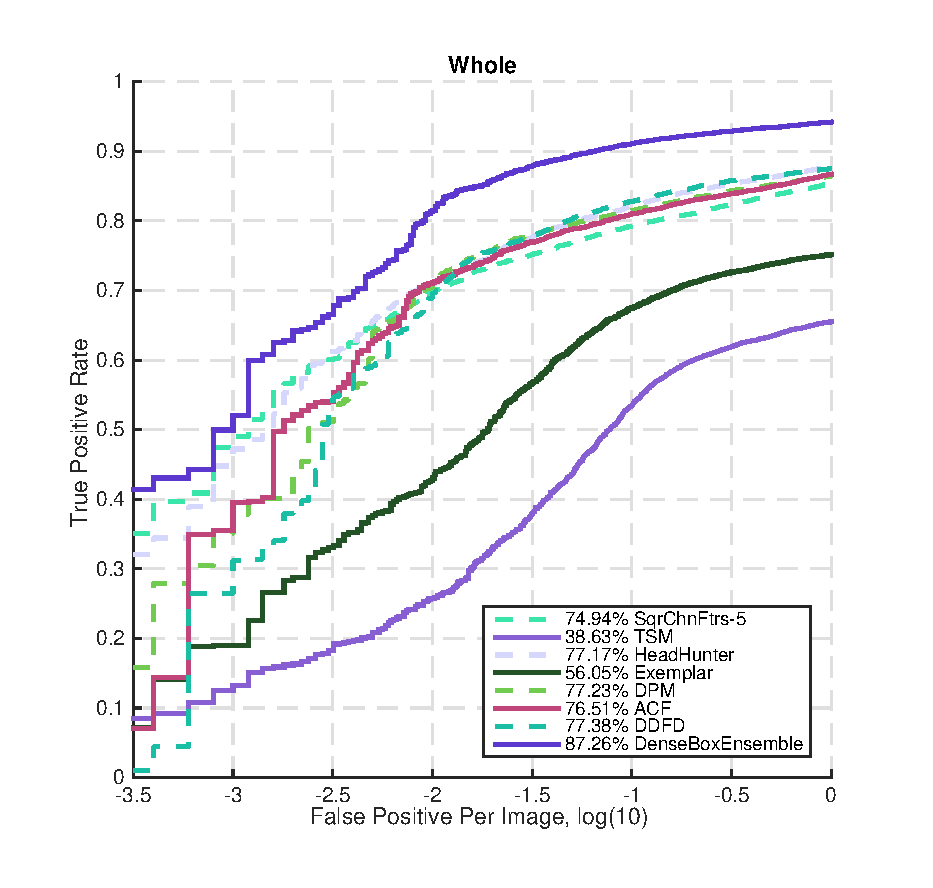
\includegraphics[scale = 0.5]{figures/MALF_2.eps}  (b)
  \end{minipage} 
 \caption{  \textbf{Result on MALF dataset. }  (a) Comparison of different versions of DenseBox; (b)The curves and mean recall rate of DenseBox and other methods;  }\label{fig:fig_malf}
\end{figure}

 
\subsection{ KITTI Car Detection Task}
The KITTI object detection benchmark consists of 7481 training images and 7518 test images. The total number of objects in training sums up to 51,867, in which cars only accounts for 28,742. The key difficulty of KITTI car detection task is that a great amount of cars are in small size (height < 40 pixels) and occluded.  To overcome this difficulty,  previous works such as\cite{li2014integrating} need careful part and occlusion modeling. 

\textbf{Training and Testing.} As well as in face detection task, we train two models(one without landmark, the other with landmark) on the KITTI object detection training set. Since KITTI does not provide landmarks for car, we selectively annotate 8 landmarks for large cars (height > 50 pixels). The landmarks of car is shown in Fig \ref{fig:fig_landmark}, and we finally annotate 7790 cars, roughly $27\%$ of the total cars. The testing procedure is the same as in face detection, except that we do not down sample car images. The evaluation metric of KITTI car detection task is different from general objecte detection. KITTI requires an overlap of 70\% for true positive bounding box, while other tasks such as face detection only requires 50\% overlap. This strict criteria requests high accurate car localization. On KITTI, we set the non-maximum suppression  IOU threshold to 0.75. 

\textbf{Results.} 

	\renewcommand{\arraystretch}{1.5}
	\begin{table}[!hbt]
	\centering
	\begin{tabular}{|l|c|c|c|}
	\hline

	Method & \textit{Moderate} &\textit{Easy} & \textit{Hard}\\
	\hline
	Regionlets~\cite{long2015accurate}	 &76.45\%	  &84.75\%	  &59.70\% 	 \\ 
	AOG~\cite{li2014integrating}	&74.26\%	&84.24\% 		&60.51\% \\
	3DVP~\cite{xiang2015data}			&75.77\%	&87.46\%	&65.38\%       \\
	spCov\_LBP 	&77.40\%	&87.19\%	&60.60\%   \\
	DeepInsight	&84.40\%	&84.59\%	&76.09\%     \\
	NIPS ID 331	&87.14\%	&88.33\%	&76.11\% \\
	DJML	&88.79\%	&91.31\%	&77.73\% \\
	\hline
	
	\hline
	DenseBox (without landmark)	&85.07\%	&82.33\%	&76.27\%   \\
	DenseBox (withlandmark)		&85.74\%	&83.63\%	&76.71\%     \\
 
	\hline
	\end{tabular}
	\caption{The Averate Presision on KITTI Car Detection Task} 
	\label{tab:tab_kitti}
	\end{table}

\textbf{Results.} Table \ref{tab:tab_kitti} shows the results of DenseBox and other methods. We can see that partially annotated landmark information (27\%) still can boost detection performance. On average, model with landmark localization slightly outperforms no-landmark model by 0.9\% in average precision.  The promotion on performance is not as great as in face detection.  The reason could be that the landmark information is not sufficient.  The insufficient lies on both the amount (27\% in car while 100\% in face) and the quality (8 landmarks in car whereas 74 in face). Compared with other methods, the DenseBox still achieves competitive results.  DenseBox defeats traditional detection system such as Regionlets and spCov by a large margin. Our average precision on moderate car is 85.74\%, slightly better than DeepInsight, which use R-CNN framework with ImageNet pre-trained GoogLeNet\cite{szegedy2014going}.  Our model has been ranked as the top 1 for 4 months until an anonymous submission titled  ``NIPS ID 331’’, which use stereo information for training and testing. Recently a method named ``DJML’’ overtakes all other methods. 

	\begin{figure}[!hbtp]
	\centering
	 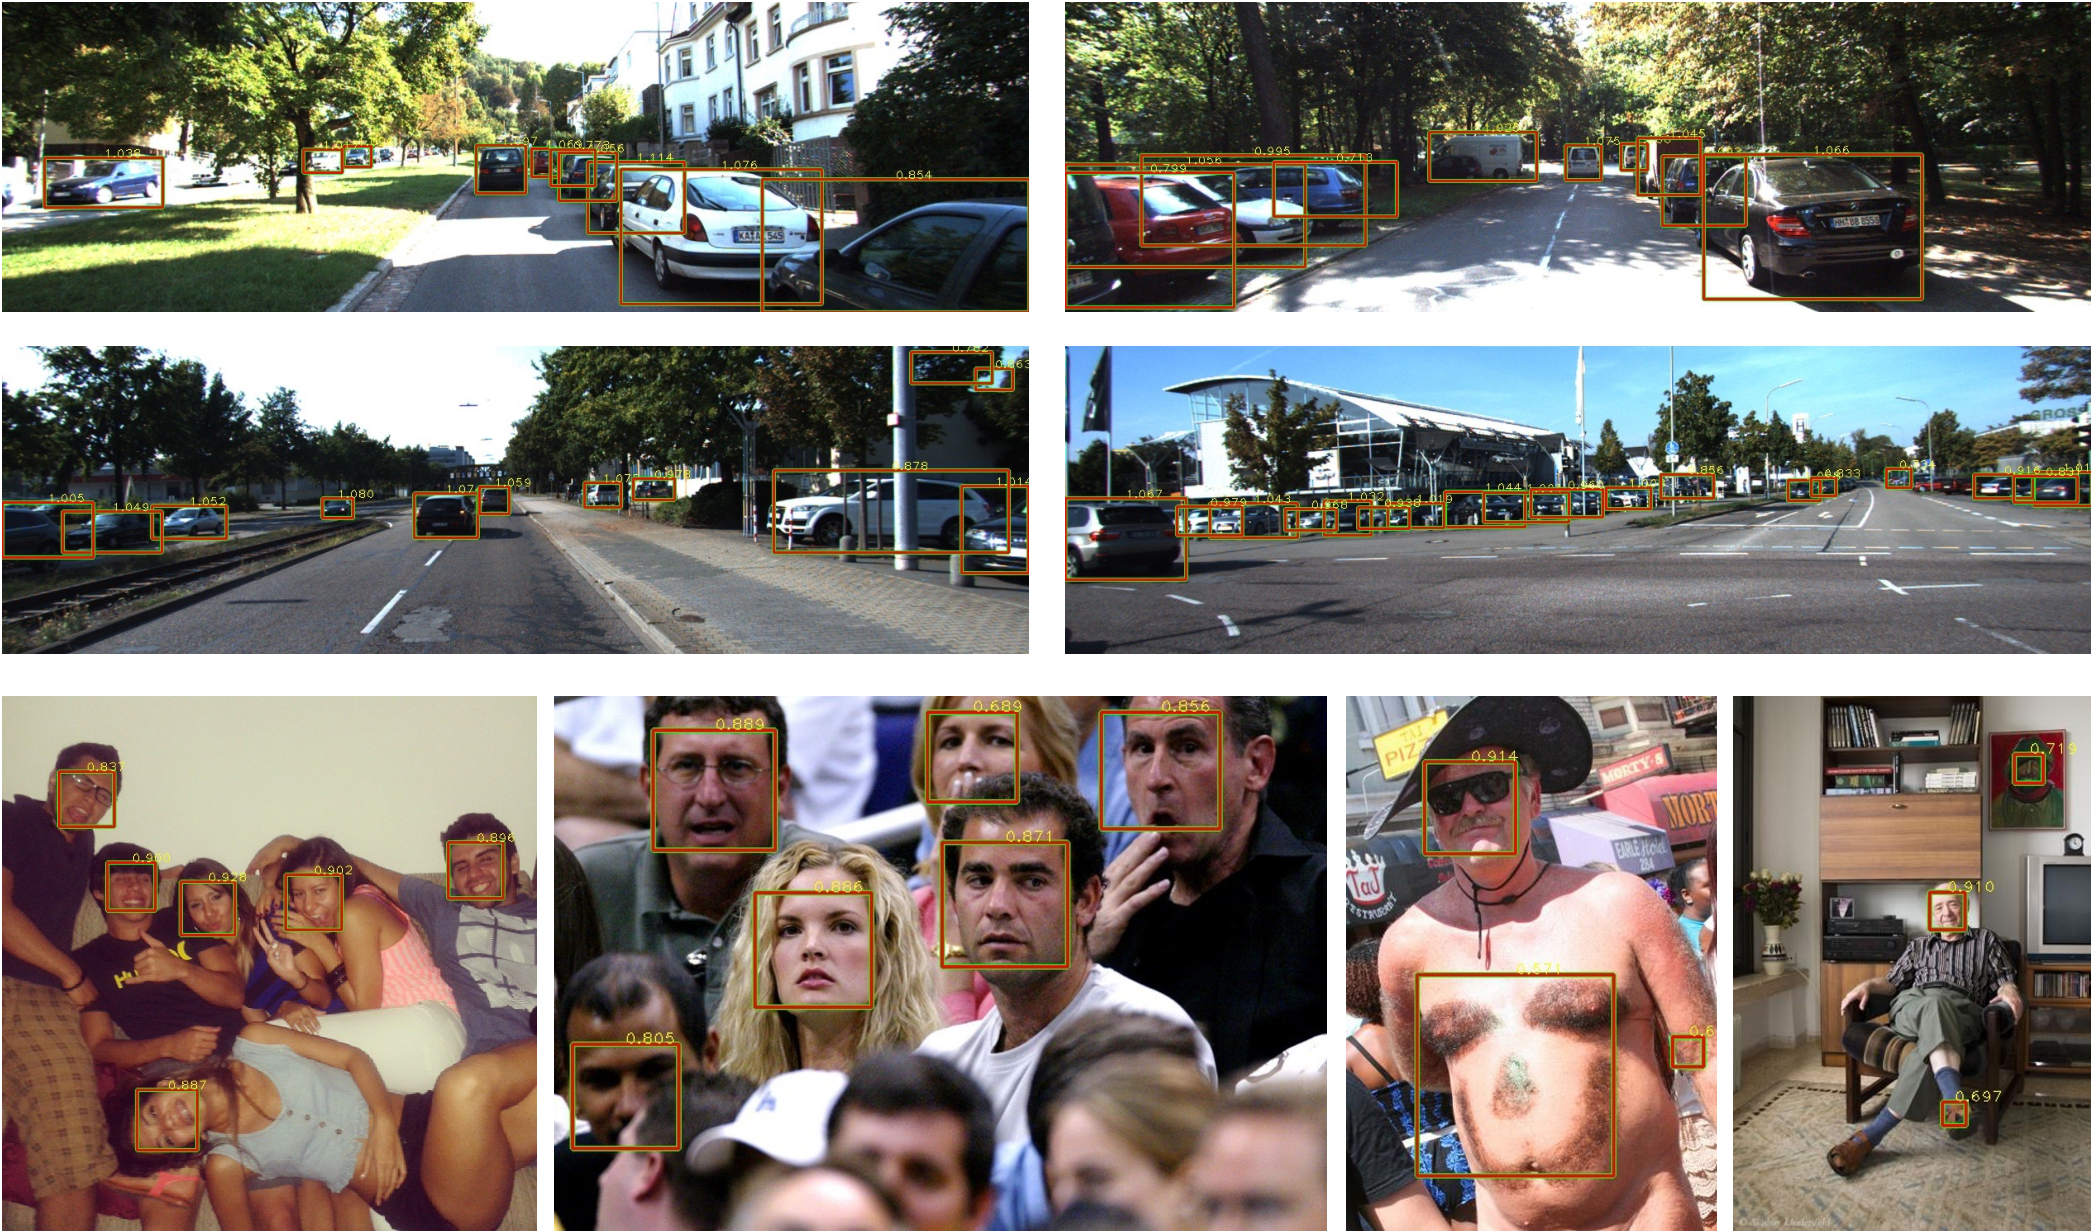
\includegraphics[scale=0.4]{figures/figure5-crop.pdf}
	\caption{\textbf{Examples on both the MALF detection set KITTI car detection set. }The numbers above the bounding boxes are the confidence score. Our system works very well in complex scene where objects are small and highly occluded. However, it still could miss some objects and generate false alarm.     }
	\label{fig:fig_case}
	\end{figure}
\section{Conclusion}

We have presented the DenseBox, a unified end-to-end detection pipeline for detection. The performance can be boosted easily by incorporating landmark information. We also analysis our method and other related object detection system, highlighting the difference and the contribution of DenseBox.  The DenseBox achieves impressive performance on both face detection and car detection task, demonstrating its high suitable for situation where proposal generation might fail. The key problem of DenseBox is the speed.  The original DenseBox presented in this paper needs several seconds to process one image. But this has been addressed in our latter version.  We will present another paper describing a real-time detection system on KITTI and face detection, called DenseBox2.  


